\subsection{Results for $x$ Offset}
%\label{subsec:longitude_no_abs_results}
%\vspace{10pt}

Figure~\ref{fig:var_long} represents the $p$-values for the Wilcoxon signed-rank test on actual and predicted values across $k$-fold validation datasets for the $x$ offset in the $k$-fold testing datasets using different RNN models, and forecasting times. Darker colors in grayscale represent a higher $p$-value in a range from $0$ to $1$. The values on the secondary diagonal are all equal to $1$ and black because models equal themselves.

\begin{figure}[!ht]
	\centering
	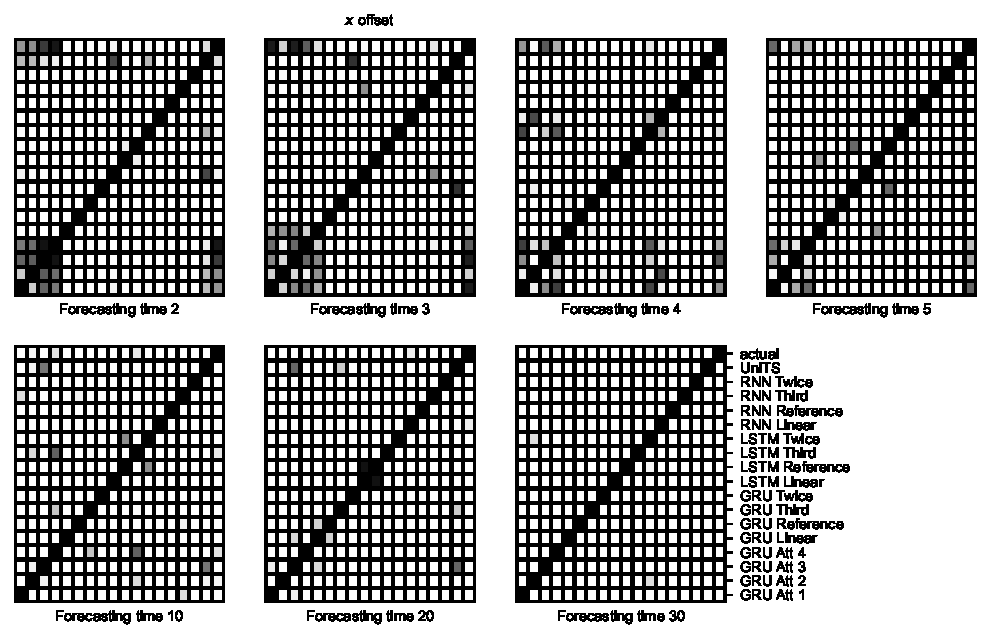
\includegraphics[width = 0.99 \linewidth]{var_long.pdf}
	\caption{The $p$-values for the Wilcoxon signed-rank test on actual and predicted values across $k$-fold validation datasets for the $x$ offset in the $k$-fold testing datasets using different RNN models, and forecasting times. Darker colors in grayscale represent a higher $p$-value in a range from $0$ to $1$. The values on the secondary diagonal are all equal to $1$ and black because models equal themselves.}
	\label{fig:var_long}
\end{figure}

The average RMSE ($\times 10^{-4}$), with standard deviation in brackets, across $k$-fold validation datasets for the $x$ offset estimated on the $k$-fold testing datasets by different RNN models, and forecasting times is listed in Table~\ref{tab:best_longitude_no_abs_RMSE}.

\begin{table}[!ht]
	\centering
	\resizebox{\linewidth}{!}{
		\begin{tabular}{|c|c|c|c|c|c|c|c|}
			\hline
			Model & $2$ $s$ & $3$ $s$ & $4$ $s$ & $5$ $s$ & $10$ $s$ & $20$ $s$ & $30$ $s$ \\ \hline
			\multirow{2}{*}{GRU Att 1} & $1.4$ & $\mathbf{1.85}$ & $2.26$ & $2.54$ & $4.54$ & $6.05$ & $6.47$ \\
			 & ($0.19$) & \textbf{(}$\mathbf{0.24}$\textbf{)} & ($0.27$) & ($0.27$) & ($0.69$) & ($0.47$) & ($0.6$) \\ \hline
			\multirow{2}{*}{LSTM Third} & $\mathbf{1.12}$ & $2.01$ & $2.6$ & $3.14$ & $4.7$ & $6.57$ & $7.27$ \\
			 & \textbf{(}$\mathbf{0.2}$\textbf{)} & ($0.38$) & ($0.37$) & ($0.36$) & ($0.41$) & ($0.48$) & ($0.43$) \\ \hline
			\multirow{2}{*}{UniTS} & $1.58$ & $1.92$ & $\mathbf{2.22}$ & $\mathbf{2.49}$ & $\mathbf{3.57}$ & $\mathbf{4.89}$ & $\mathbf{5.65}$ \\
			 & ($0.18$) & ($0.2$) & \textbf{(}$\mathbf{0.22}$\textbf{)} & \textbf{(}$\mathbf{0.24}$\textbf{)} & \textbf{(}$\mathbf{0.32}$\textbf{)} & \textbf{(}$\mathbf{0.4}$\textbf{)} & \textbf{(}$\mathbf{0.43}$\textbf{)} \\ \hline
		\end{tabular}
	}
	\caption{The average RMSE ($\times 10^{-4}$), with standard deviation in brackets, across $k$-fold validation datasets for the $x$ offset estimated on the $k$-fold testing datasets by different RNN models, and forecasting times.}
	\label{tab:best_longitude_no_abs_RMSE}
\end{table}

The GRU Att 1 model achieved the lowest RMSE for $x$ offset, and a forecasting time of $3$ $s$ with an average value and standard deviation (in brackets) that equals $18.46 \times 10^{-5}$ $\degree$ ($2.4 \times 10^{-5}$ $\degree$).

The GRU Att 1 model does not have a statistically significantly different RMSE than the GRU Att 2, GRU Third, GRU Twice, LSTM Linear, LSTM Third, LSTM Twice, RNN Third, and UniTS models for $x$ offset using a forecasting time of $3$ $s$, with $p$-values equaling $1.073 \times 10^{-1}$, $2.255 \times 10^{-3}$, $4.605 \times 10^{-3}$, $5.564 \times 10^{-4}$, $2.027 \times 10^{-2}$, $9.789 \times 10^{-1}$, $3.764 \times 10^{-4}$, and $7.15 \times 10^{-4}$.

\markertable{tab:\label{tab:RMSE:longitude:no:abs:p:3}}

The LSTM Third model achieved the lowest RMSE for $x$ offset, and a forecasting time of $2$ $s$ with an average value and standard deviation (in brackets) that equals $11.23 \times 10^{-5}$ $\degree$ ($2.01 \times 10^{-5}$ $\degree$).

The LSTM Third model does not have a statistically significantly different RMSE than the GRU Linear, GRU Third, GRU Twice, LSTM Linear, and LSTM Reference models for $x$ offset using a forecasting time of $2$ $s$, with $p$-values equaling $6.313 \times 10^{-4}$, $7.112 \times 10^{-1}$, $5.424 \times 10^{-1}$, $6.263 \times 10^{-2}$, and $2.027 \times 10^{-2}$.

\markertable{tab:\label{tab:RMSE:longitude:no:abs:p:2}}

The UniTS model achieved the lowest RMSE for $x$ offset, and a forecasting time of $4$, $5$, $10$, $20$, and $30$ $s$ with average values and standard deviation (in brackets) that equal $22.19 \times 10^{-5}$ $\degree$ ($2.24 \times 10^{-5}$ $\degree$), $24.94 \times 10^{-5}$ $\degree$ ($2.44 \times 10^{-5}$ $\degree$), $35.65 \times 10^{-5}$ $\degree$ ($3.19 \times 10^{-5}$ $\degree$), $48.95 \times 10^{-5}$ $\degree$ ($4.04 \times 10^{-5}$ $\degree$), and $56.54 \times 10^{-5}$ $\degree$ ($4.33 \times 10^{-5}$ $\degree$) respectively.

The UniTS model does not have a statistically significantly different RMSE than the GRU Att 1, and GRU Att 2 models for $x$ offset using a forecasting time of $4$ $s$, with $p$-values equaling $5.875 \times 10^{-2}$, and $1.908 \times 10^{-1}$.

\markertable{tab:\label{tab:RMSE:longitude:no:abs:p:4}}

The UniTS model does not have a statistically significantly different RMSE than the GRU Att 1, and GRU Att 2 models for $x$ offset using a forecasting time of $5$ $s$, with $p$-values equaling $2.748 \times 10^{-2}$, and $9.032 \times 10^{-2}$.

\markertable{tab:\label{tab:RMSE:longitude:no:abs:p:5}}

